\documentclass[12pt]{beamer}
\usetheme{Warsaw}
\usepackage[utf8]{inputenc}
\usepackage{amsmath}
\usepackage{amsfonts}
\usepackage{amssymb}
\usepackage{graphicx}
\usepackage[font=Times,timeinterval=1,timeduration=2.0,timedeath=0,fillcolorwarningsecond=white!60!yellow,timewarningfirst=50,timewarningsecond=80,resetatpages=2]{tdclock}
\usepackage{tabularx}
\usepackage{array}
\usepackage{multicol}
\usepackage{longtable}
\usepackage{xcolor}
\usepackage{gensymb}
\usepackage{pgfplots}

\graphicspath{ {./references/} }
\pgfplotsset{
	soldot/.style={color=black,only marks,mark=*},
	holdot/.style={color=black,fill=white,only marks,mark=*},
	compat=1.12
}
\newcolumntype{Y}{>{\centering\arraybackslash}X} % *: Beamer enumeration spacing-workaround..
\makeatletter
\def\@listii{\leftmargin\leftmarginii
			  \topsep    2ex
			  \parsep    0\p@   \@plus\p@
			  \itemsep   \parsep}
\makeatother

\begin{document}
\begin{frame}
	\frametitle{Bellwork 9/13}
	\large
	\vspace*{\fill}
	\vspace*{\fill}
	\initclock
	\begin{enumerate}
		\item Evaluate \[\displaystyle\lim_{x\to5}\left(\frac{x^2+x-30}{5-x}\right)\]
		      \vspace*{\fill}
		\item Find $\displaystyle\lim_{x\to0}f(x)$ where
		      \[
			      f(x) =
			      \begin{cases}
				      \sqrt{4-x} & \text{if } x < 0    \\
				      x+2        & \text{if } x \geq 0 \\
			      \end{cases}
		      \]\\
	\end{enumerate}
	\vspace*{\fill}
	\vspace*{\fill}
	\crono
	\resetcrono{\beamerbutton{reset}}
\end{frame}
\begin{frame}
	\frametitle{Bellwork 9/13 - Solutions}
	\begin{enumerate}\itemsep2ex
		\large
		\item \[\displaystyle\lim_{x\to5}\left(\frac{x^2+x-30}{5-x}\right)=\boxed{-11}\]
		\item
		      \[
			      f(x) =
			      \begin{cases}
				      \sqrt{4-x} & \text{if } x < 0    \\
				      x+2        & \text{if } x \geq 0 \\
			      \end{cases}
		      \]
		      \vspace*{\fill}
		      \begin{table}[]
			      $\displaystyle\lim_{x\to0^{-}}f(x)=2$
			      \hspace{0.25cm}
			      $\displaystyle\lim_{x\to0^{+}}f(x)=2$
		      \end{table}
		      \[\implies\displaystyle\lim_{x\to0}f(x) = \boxed{2}\]
	\end{enumerate}
\end{frame}
\begin{frame}
	\frametitle{Exercise 1}
	\vspace*{\fill}
	\vspace*{\fill}
	\initclock
	\large
	\begin{minipage}{0.5\textwidth} % TODO: Add equal spacing between the minipages.
		\begin{center} % Are these redundant?
			$f(2) = 3$\\
			$g(2) = -6$\\
			$h(2) = -3$
		\end{center}
	\end{minipage}%
	\begin{minipage}{0.5\textwidth}
		\begin{center}
			$\displaystyle\lim_{x\to2}f(x) = 4$\\
			$\displaystyle\lim_{x\to2}g(x) = -6$\\
			$\displaystyle\lim_{x\to2}h(x) = 2$ % ?: Was it x\to7 or was that a written mistake?
		\end{center}
	\end{minipage}\\
	\vspace*{\fill}
	\begin{center}
		What is $\displaystyle\lim_{x\to2}[h(x)(5f(x)+g(x))]$?\\
	\end{center}
	\vspace*{\fill}
	\vspace*{\fill}
	\crono
	\resetcrono{\beamerbutton{reset}}
\end{frame}
\begin{frame}
	\frametitle{Exercise 1 - Solution}
	Since all of the limits are defined, we can directly rewrite the expression and substitute:
	\[\displaystyle\lim_{x\to2}[h(x)(5f(x)+g(x))]\]
	\[= \displaystyle\lim_{x\to2}h(x)\cdot\left[5\displaystyle\lim_{x\to2}f(x)+\displaystyle\lim_{x\to2}g(x)\right]\]
	\[= 2(5\cdot4 - 6)\]
	\[= \boxed{28}\]

\end{frame}
\begin{frame}
	\frametitle{Exercise 2}
	\initclock
	\begin{center}
		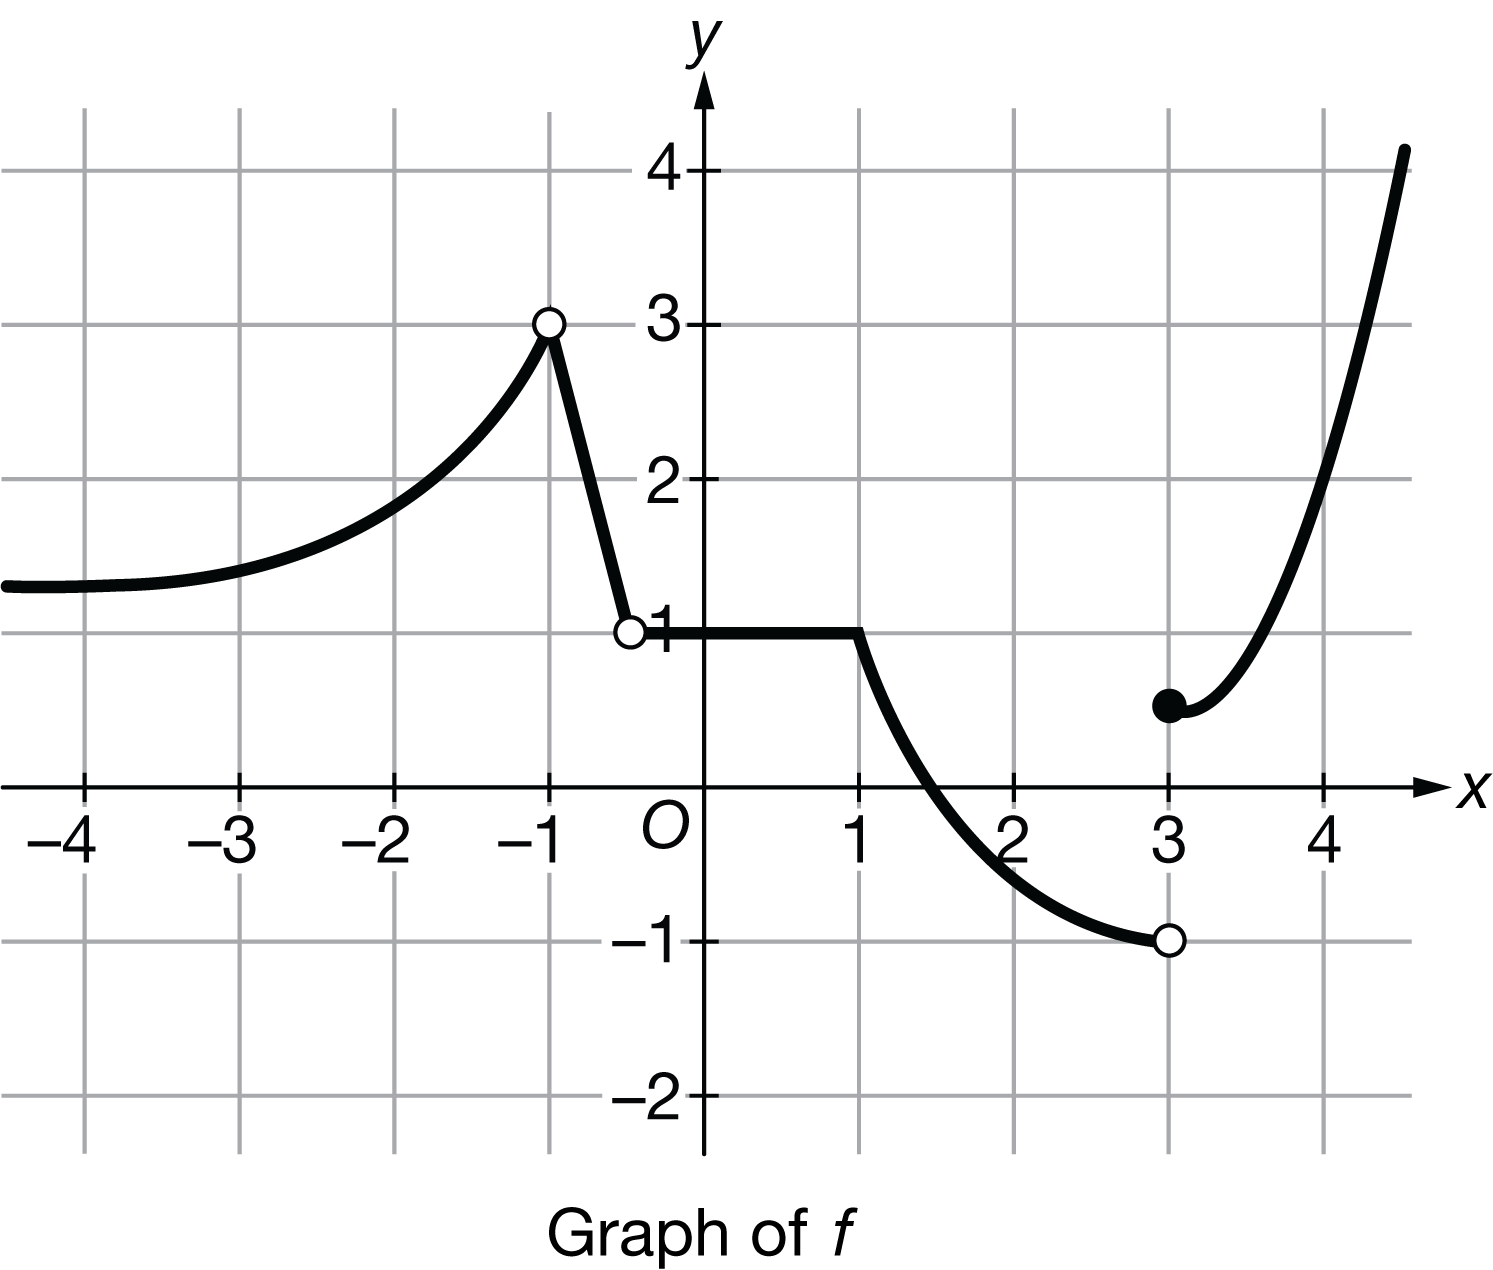
\includegraphics[scale=0.5]{graph0913.png}
	\end{center}
	\large
	\begin{center}
		What is $\displaystyle\lim_{x\to-1}f[f(x)]$?\\
	\end{center}
	\crono
	\resetcrono{\beamerbutton{reset}}
\end{frame}
\begin{frame}
	\frametitle{Exercise 2 - Solution}

	\[\displaystyle\lim_{x\to-1}f(x) = 3\]
	\[\implies\displaystyle\lim_{x\to-1}f[f(x)]\]
	\[=\]
\end{frame}
\end{document}